\documentclass[a4paper]{scrreprt}

\usepackage[ngerman]{babel}
\usepackage[utf8]{inputenc}
\usepackage{pslatex}
\usepackage{amssymb}
\usepackage{textcomp}
\usepackage{parskip}
\usepackage{graphicx}
\usepackage{txfonts}
\usepackage[T1]{fontenc}
\usepackage{user} % eigene Befehle
\usepackage{longtable}
\usepackage{floatflt}
\usepackage{listings}

\ifpdf
  \usepackage[ps2pdf]{thumbpdf}
  \usepackage[pdftex]{hyperref}
\else
  \usepackage[active]{srcltx}
\fi

% Einstellung für Listings
\lstset{numbers=left, numberstyle=\tiny, numbersep=5pt, basicstyle=\scriptsize, showstringspaces=false}
\lstset{language=PHP, inputencoding=latin1, breaklines=true, breakatwhitespace=true}

\newcommand{\dctitle}{Literaturverwaltung}
\newcommand{\dcsubject}{Projektdokumentation}
\newcommand{\dcsubtitle}{Teilbeleg 1}
\newcommand{\dcauthor}{Simon Wunderlich}
\newcommand{\dcdate}{\today}

\ifpdf
\hypersetup{%
   pdfauthor={\dcsubject - \dcauthor}
   pdftitle={\dctitle}
   bookmarksnumbered=true,
   pdfstartview={FitH},
   colorlinks=true,
   linkcolor=black,
   plainpages = false
}
\fi
 % Metainformationen wie Titel, Autoren,...

\begin{document}
% Momentan (schlecht) handgestrickt - wenn jemand es mit \maketitle und den
% Autoren wie in Vorlage hinbekommt, bitte ändern

\begin{titlepage}
	\begin{center}\sffamily
		\vspace{15mm}
		
\includegraphics{tuclogo}
		\vfill
		{% Kopf des Titels
			\large Softwarepraktikum 2006\\[1.5ex]
		}
		\vfill \vfill

		%Titel
		\textbf{\Huge\dctitle}
		\vspace{1.5cm}
		
		% Subjekt
		\textbf{\Large\dcsubject}

		% Untertitel
		\textsc{\Large \dcsubtitle}
		\vfill \vfill
	\end{center}
	
	
	{%Autoren
		\begin{tabbing}
			\hspace{4.5cm}\=\textbf{Teamleiter:}\hspace{0.5cm}\=Simon~Wunderlich\\[2.0ex]
				\>\textbf{Mitglieder des Projektteams:}\\[1.5ex]
				\>            \>Andreas~Tröger \\[1.5ex]
				\>            \>Benedikt~Keil \\[1.5ex]
				\>            \>Frank~Wilhelm \\[1.5ex]
				\>            \>Florian~Scharl \\[1.5ex]
				\>            \>Sven~Eckelmann \\[4.0ex]
				\> \textbf{Praktikumsbetreuer:} Michael Rentzsch
		\end{tabbing}
	}
	\vfill
	
	{%Betreuer
		Chemnitz, den \dcdate
	}
\end{titlepage}
 % Titel des Dokuments mit Informationen aus meta
\cleardoublepage
\tableofcontents
\cleardoublepage

%Kapitel
\chapter{Programmdokumentation}
% Während der Weiteren Arbeiten kurzzeitig deaktiviert
% Klasseninterfaces
\section{Definition Klasseninterfaces}
\subsection{Klasse Autor}
\lstinputlisting{interfaces/autor.php}

\subsection{Klasse Kommentar}
\lstinputlisting{interfaces/kommentar.php}

\subsection{Klasse LiteraturArt}
\lstinputlisting{interfaces/literaturart.php}

\subsection{Klasse Literatur}
\lstinputlisting{interfaces/literatur.php}

\subsection{Klasse Login}
\lstinputlisting{interfaces/login.php}

\subsection{Klasse Mitglied}
\lstinputlisting{interfaces/mitglied.php}

\subsection{Klasse SQLDB}
\lstinputlisting{interfaces/sqldb_mysql.php}

\subsection{Klasse Suche}
\lstinputlisting{interfaces/suche.php}

% Quelltexte
\section{Kommentierte Quelltexte}
\subsection{bibtex.php}
\lstinputlisting{sourcecodes/bibtex.php}

\subsection{commentmod.php}
\lstinputlisting{sourcecodes/commentmod.php}

\subsection{index.php}
\lstinputlisting{sourcecodes/index.php}

\subsection{install.php}
\lstinputlisting{sourcecodes/install.php}

\subsection{litmod.php}
\lstinputlisting{sourcecodes/litmod.php}

\subsection{lit.php}
\lstinputlisting{sourcecodes/lit.php}

\subsection{login.php}
\lstinputlisting{sourcecodes/login.php}

\subsection{searchmore.php}
\lstinputlisting{sourcecodes/searchmore.php}

\subsection{search.php}
\lstinputlisting{sourcecodes/search.php}

\subsection{userlist.php}
\lstinputlisting{sourcecodes/userlist.php}

\subsection{usermod.php}
\lstinputlisting{sourcecodes/usermod.php}

\subsection{user.php}
\lstinputlisting{sourcecodes/user.php}

\subsection{design/liman.css}
\lstinputlisting{sourcecodes/design/liman.css}

\subsection{include/autor.php}
\lstinputlisting{sourcecodes/include/autor.php}

\subsection{include/config.php}
\lstinputlisting{sourcecodes/include/config.php}

\subsection{include/footer.php}
\lstinputlisting{sourcecodes/include/footer.php}

\subsection{include/form\_helper.php}
\lstinputlisting{sourcecodes/include/form_helper.php}

\subsection{include/global.php}
\lstinputlisting{sourcecodes/include/global.php}

\subsection{include/header.php}
\lstinputlisting{sourcecodes/include/header.php}

\subsection{include/kommentar.php}
\lstinputlisting{sourcecodes/include/kommentar.php}

\subsection{include/literaturart.php}
\lstinputlisting{sourcecodes/include/literaturart.php}

\subsection{include/literatur.php}
\lstinputlisting{sourcecodes/include/literatur.php}

\subsection{include/login.php}
\lstinputlisting{sourcecodes/include/login.php}

\subsection{include/mitglied.php}
\lstinputlisting{sourcecodes/include/mitglied.php}

\subsection{include/sqldb\_mysql.php}
\lstinputlisting{sourcecodes/include/sqldb_mysql.php}

\subsection{include/sqldb.php}
\lstinputlisting{sourcecodes/include/sqldb.php}

\subsection{include/suche.php}
\lstinputlisting{sourcecodes/include/suche.php}


% Tests
\section{Testplan}
\subsection{Testfälle}

\subsubsection{Fall 1: Unit Tests}
\begin{enumerate}
\item Systemzustand vor dem Test:\\
	TODO: Hübsche Formulierung für: egal, wird nicht benutzt
\item Eingabedaten:\\
	test.php wird aufgerufen. Sonstige Eingaben werden fest im Code der Tests durchgeführt.
\item Erwartete Ereignisse:\\
	Alle Tests liefern "OK" zurück
\item Systemzustand nach Test:\\
	Unverändert, wie vor dem Test.
\end{enumerate}

\subsubsection{Fall 2: Installation}
\begin{enumerate}
\item Systemzustand vor dem Test:\\
	1. Durchlauf: Alle Speicher nicht vorhanden, aber die Datenbank. 2. Durchlauf: Speicher sind vorhanden und mit zufälligen Werten gefüllt.
\item Eingabedaten:\\
	install.php wird aufgerufen und die verlangten Daten eingegeben.
\item Erwartete Ereignisse:\\
	Verbindung mit Datenbank wird erstellt, schon vorhandene Speicher gelöscht, Speicher neu angelegt und neuer Administrator angelegt
\item Systemzustand nach Test:\\
	Leere Speicher Autoren, Bibliothek, Kommentare und Literatur\_Autoren bestehen. Außerdem existiert Speicher Mitglieder mit einem Datensatz (Administrator Admin Istrator mit angegebenen Login und gehashtem Passwort)
\end{enumerate}

\subsubsection{Fall 3: Test des Nutzerinterfaces -- Administrator}
\begin{enumerate}
\item Systemzustand vor dem Test:\\
	Alle Speicher bis auf Mitglieder sind leer. In Mitglieder ist nur der Datensatz des ersten Administrators.
\item Eingabedaten:\\
	Begonnen wird der Test mit dem Anmelden als Administrator. Alle Funktionen des Systems werden nacheinander aktiviert, ohne Eintragungen vorzunehmen. Beendet wird der Test mit dem Abmelden.
\item Erwartete Ereignisse:\\
	Korrekte Anzeige der entsprechend der aktivierten Aktion laut Layoutentwurf zugeordneten Ansicht.
\item Systemzustand nach Test:\\
	Unverändert, wie vor dem Test.
\end{enumerate}

\subsubsection{Fall 4: Test des Nutzerinterfaces -- Benutzer}
\begin{enumerate}
\item Systemzustand vor dem Test:\\
	Alle Speicher bis auf Mitglieder sind leer. In Mitglieder ist neben dem Datensatz des ersten Administrators ein Mitglied ohne Administratorrechte vorhanden.
\item Eingabedaten:\\
	Begonnen wird der Test mit dem Anmelden als Mitglied. Alle Funktionen des Systems werden nacheinander aktiviert, ohne Eintragungen vorzunehmen. Beendet wird der Test mit dem Abmelden.
\item Erwartete Ereignisse:\\
	Korrekte Anzeige der entsprechend der aktivierten Aktion laut Layoutentwurf zugeordneten Ansicht. Die Nutzerliste zeigt nur den eigenen Nutzereintrag an. Jegliche Provokation des Systems (Löschen und Hinzufügen eines Mitglieds und das Bearbeiten eines fremden Mitglieds) wird abgewiesen bzw. auf die eigenen Nutzerdaten umgeleitet.
\item Systemzustand nach Test:\\
	Unverändert, wie vor dem Test.
\end{enumerate}

\subsubsection{Fall 5: Test des Nutzerinterfaces -- Gast}
\begin{enumerate}
\item Systemzustand vor dem Test:\\
	Alle Speicher bis auf Mitglieder sind leer. In Mitglieder ist nur der Datensatz des ersten Administrators.
\item Eingabedaten:\\
	Nutzer ist nicht angemeldet. Alle Funktionen des Systems werden nacheinander aktiviert, ohne Eintragungen vorzunehmen.
\item Erwartete Ereignisse:\\
	Korrekte Anzeige der entsprechend der aktivierten Aktion laut Layoutentwurf zugeordneten Ansicht. Es sind keine Elemente zum Hinzufügen, Ändern oder Löschen von Daten vorhanden. Die Nutzerliste zeigt keinen Nutzereintrag an. Jegliche Provokation des Systems (Löschen und Hinzufügen, Ändern eines Mitglieds, Kommentars, Literatur) wird abgewiesen.
\item Systemzustand nach Test:\\
	Unverändert, wie vor dem Test.
\end{enumerate}

\subsubsection{Fall 6: Anlegen neue Literatur}
\begin{enumerate}
\item Systemzustand vor dem Test:\\
	Alle Speicher bis auf Mitglieder sind leer. In Mitglieder ist neben dem Datensatz des ersten Administrators ein Mitglied ohne Administratorrechte vorhanden.
\item Eingabedaten:\\
	Begonnen wird der Test mit dem Anmelden als Mitglied. Neue Literatur wird angelegt. Beendet wird der Test mit dem Abmelden.
\item Erwartete Ereignisse:\\
	System legt neue Literatur an und gibt Erfolgsmeldung aus.
\item Systemzustand nach Test:\\
	Alle Speicher bis auf Bibliothek sind unverändert. In Bibliothek existiert ein korrekter Datensatz.
\end{enumerate}

\subsubsection{Fall 7: Anlegen neue Literatur, die schon existiert}
\begin{enumerate}
\item Systemzustand vor dem Test:\\
	Alle Speicher bis auf Mitglieder und Bibliothek sind leer. In Mitglieder ist neben dem Datensatz des ersten Administrators ein Mitglied ohne Administratorrechte vorhanden. In Bibliothek sind mehrere Literaturdatensätze vorhanden.
\item Eingabedaten:\\
	Begonnen wird der Test mit dem Anmelden als Mitglied. Neue Literatur wird angelegt mit ähnlichen/gleichen Daten wie eine existierende Literatur angelegt. Anlegen wird bestätigt. Beendet wird der Test mit dem Abmelden.
\item Erwartete Ereignisse:\\
	System fragt ob die Literatur angelegt werden soll und zeigt Liste der ähnlichen Literatur an. Nach Bestätigung legt das System neue Literatur an und gibt Erfolgsmeldung aus.
\item Systemzustand nach Test:\\
	Alle Speicher bis auf Bibliothek, Literatur\_Autoren und Autoren sind unverändert. In Bibliothek existiert ein neuer korrekter Datensatz, in Autoren sind angegebene Autoren eingefügt und in Literatur\_Autoren sind die Verbindung von Literatur zu Autoren vorhanden.
\end{enumerate}

\subsubsection{Fall 8: Ändern Literatur}
\begin{enumerate}
\item Systemzustand vor dem Test:\\
	Kommentare ist leer. In Mitglieder ist neben dem Datensatz des ersten Administrators ein Mitglied ohne Administratorrechte vorhanden. In Bibliothek sind mehrere Literaturdatensätze vorhanden. In Autoren sind Autoren vohanden und in Literatur\_Autoren sind die Verbindungen zu Literatur vorhanden.
\item Eingabedaten:\\
	Begonnen wird der Test mit dem Anmelden als Mitglied. Bestehende Literatur wird gewählt und bearbeitet. Beendet wird der Test mit dem Abmelden.
\item Erwartete Ereignisse:\\
	System ändert Literatur und gibt Erfolgsmeldung aus.
\item Systemzustand nach Test:\\
	Alle Speicher bis auf Bibliothek, Literatur\_Autoren und Autoren sind unverändert. In Bibliothek existiert die selbe Anzahl an Datensätzen und der zu ändernte Datensatz wurde korrekt überschrieben. In Autoren sind angegebene Autoren eingefügt, nicht angegebene entfernt und in Literatur\_Autoren sind die Verbindung von Literatur zu Autoren vorhanden.
\end{enumerate}

\subsubsection{Fall 9: Löschen Literatur}
\begin{enumerate}
\item Systemzustand vor dem Test:\\
	Kommentare ist leer. In Mitglieder ist neben dem Datensatz des ersten Administrators ein Mitglied ohne Administratorrechte vorhanden. In Bibliothek sind mehrere Literaturdatensätze vorhanden. In Autoren sind Autoren vohanden und in Literatur\_Autoren sind die Verbindungen zu Literatur vorhanden.
\item Eingabedaten:\\
	Begonnen wird der Test mit dem Anmelden als Mitglied. Bestehende Literatur wird gewählt und entfernt. Beendet wird der Test mit dem Abmelden.
\item Erwartete Ereignisse:\\
	System fragt nach Bestätigung und ändert nach Bestätigung Literatur und gibt Erfolgsmeldung aus.
\item Systemzustand nach Test:\\
	Alle Speicher bis auf Bibliothek, Literatur\_Autoren und Autoren sind unverändert. In Bibliothek existieren alle Datensätze, bis auf den zu löschenden Datensatz. In Autoren sind nicht mehr benutzte Autoren entfernt und in Literatur\_Autoren sind die nicht mehr benötigten Verbindungen von Literatur zu Autoren entfernt.
\end{enumerate}

\subsubsection{Fall 10: Anlegen neues Mitglied}
\begin{enumerate}
\item Systemzustand vor dem Test:\\
	Alle Speicher bis auf Mitglieder sind leer. In Mitglieder ist nur der Datensatz des ersten Administrators.
\item Eingabedaten:\\
	Begonnen wird der Test mit dem Anmelden als Administrator. Neues Mitglied wird angelegt. Beendet wird der Test mit dem Abmelden.
\item Erwartete Ereignisse:\\
	System legt neues Mitglied an und gibt Erfolgsmeldung aus.
\item Systemzustand nach Test:\\
	Alle Speicher bis auf Mitglieder sind unverändert. In Mitglieder existiert neben dem Administratordatensatz ein korrekter neuer Datensatz.
\end{enumerate}

\subsubsection{Fall 11: Anlegen neues Mitglied, das schon existiert}
\begin{enumerate}
\item Systemzustand vor dem Test:\\
	Alle Speicher bis auf Mitglieder sind leer. In Mitglieder ist nur der Datensatz des ersten Administrators.
\item Eingabedaten:\\
	Begonnen wird der Test mit dem Anmelden als Administrator. Neues Mitglied wird mit dem Login des Administratos angelegt. Beendet wird der Test mit dem Abmelden.
\item Erwartete Ereignisse:\\
	System gibt Fehlermeldung aus.
\item Systemzustand nach Test:\\
	Alle Speicher sind unverändert.
\end{enumerate}

\subsubsection{Fall 12: Ändern Mitglied}
\begin{enumerate}
\item Systemzustand vor dem Test:\\
	Alle Speicher bis auf Mitglieder sind leer. In Mitglieder ist neben dem Datensatz des ersten Administrators ein weiteres Mitglied vorhanden.
\item Eingabedaten:\\
	Begonnen wird der Test mit dem Anmelden als Administrator. Mitglied wird ausgewählt und bearbeitet. Beendet wird der Test mit dem Abmelden.
\item Erwartete Ereignisse:\\
	System ändert das Mitglied und gibt Erfolgsmeldung aus.
\item Systemzustand nach Test:\\
	Alle Speicher sind bis auf Mitglieder unverändert. In Mitglieder existiert die selbe Anzahl an Datensätzen und der zu ändernte Datensatz wurde korrekt überschrieben.
\end{enumerate}

\subsubsection{Fall 13: Ändern Mitglied - eigene Daten}
\begin{enumerate}
\item Systemzustand vor dem Test:\\
	Alle Speicher bis auf Mitglieder sind leer. In Mitglieder ist neben dem Datensatz des ersten Administrators ein weiteres Mitglied ohne Administratorrechte vorhanden.
\item Eingabedaten:\\
	Begonnen wird der Test mit dem Anmelden als Mitglied. Eigene Mitgliedsdaten werden ausgewählt und bearbeitet. Beendet wird der Test mit dem Abmelden.
\item Erwartete Ereignisse:\\
	System ändert das Mitglied und gibt Erfolgsmeldung aus.
\item Systemzustand nach Test:\\
	Alle Speicher sind bis auf Mitglieder unverändert. In Mitglieder existiert die selbe Anzahl an Datensätzen und der zu eigene Datensatz wurde korrekt überschrieben.
\end{enumerate}

\subsubsection{Fall 14: Löschen Mitglied}
\begin{enumerate}
\item Systemzustand vor dem Test:\\
	Alle Speicher bis auf Mitglieder sind leer. In Mitglieder ist neben dem Datensatz des ersten Administrators ein weiteres Mitglied vorhanden.
\item Eingabedaten:\\
	Begonnen wird der Test mit dem Anmelden als Administrator. Mitglied wird ausgewählt und entfernt. Beendet wird der Test mit dem Abmelden.
\item Erwartete Ereignisse:\\
	System löscht das Mitglied und gibt Erfolgsmeldung aus.
\item Systemzustand nach Test:\\
	Alle Speicher sind bis auf Mitglieder unverändert. In Mitglieder existieren alle Datensätze, bis auf den zu löschenden Datensatz.
\end{enumerate}

\subsubsection{Fall 15: Anlegen Kommentar}
\begin{enumerate}
\item Systemzustand vor dem Test:\\
	Kommentare ist leer. In Mitglieder ist neben dem Datensatz des ersten Administrators ein Mitglied ohne Administratorrechte vorhanden. In Bibliothek ist Literaturdatensatz vorhanden. In Autoren sind Autoren vohanden und in Literatur\_Autoren sind die Verbindungen zu Literatur vorhanden.
\item Eingabedaten:\\
	Begonnen wird der Test mit dem Anmelden als Mitglied. Literatur wird ausgewählt. Neuer Kommentar wird angelegt. Beendet wird der Test mit dem Abmelden.
\item Erwartete Ereignisse:\\
	System legt neuen Kommentar an und gibt Erfolgsmeldung aus.
\item Systemzustand nach Test:\\
	Alle Speicher bis auf Kommentare sind unverändert. In Kommentare existiert ein neuer korrekter Datensatz.
\end{enumerate}

\subsubsection{Fall 16: Ändern Kommentar}
\begin{enumerate}
\item Systemzustand vor dem Test:\\
	In Mitglieder ist neben dem Datensatz des ersten Administrators ein Mitglied ohne Administratorrechte vorhanden. In Bibliothek ist Literaturdatensatz vorhanden. In Autoren sind Autoren vohanden und in Literatur\_Autoren sind die Verbindungen zu Literatur vorhanden. In Kommentare ist Kommentar zu Literatureintrag vorhanden.
\item Eingabedaten:\\
	Begonnen wird der Test mit dem Anmelden als Mitglied. Literatur wird ausgewählt. Kommentar wird geändert. Beendet wird der Test mit dem Abmelden.
\item Erwartete Ereignisse:\\
	System ändert Kommentar und gibt Erfolgsmeldung aus.
\item Systemzustand nach Test:\\
	Alle Speicher bis auf Kommentare sind unverändert. In Kommentare wurde nur der Kommentar korrekt geändert.
\end{enumerate}

\subsubsection{Fall 17: Löschen Kommentar}
\begin{enumerate}
\item Systemzustand vor dem Test:\\
	In Mitglieder ist neben dem Datensatz des ersten Administrators ein Mitglied ohne Administratorrechte vorhanden. In Bibliothek ist Literaturdatensatz vorhanden. In Autoren sind Autoren vohanden und in Literatur\_Autoren sind die Verbindungen zu Literatur vorhanden. In Kommentare sind mehrere Kommentare zu Literatureintrag vorhanden.
\item Eingabedaten:\\
	Begonnen wird der Test mit dem Anmelden als Mitglied. Literatur wird ausgewählt. Kommentar wird entfernt. Beendet wird der Test mit dem Abmelden.
\item Erwartete Ereignisse:\\
	System löscht Kommentar und gibt Erfolgsmeldung aus.
\item Systemzustand nach Test:\\
	Alle Speicher sind bis auf Kommentare unverändert. In Kommentare existieren alle Datensätze, bis auf den zu löschenden Datensatz.
\end{enumerate}

\subsubsection{Fall 18: Löschen fremden Kommentar}
\begin{enumerate}
\item Systemzustand vor dem Test:\\
	In Mitglieder ist neben dem Datensatz des ersten Administrators ein Mitglied ohne Administratorrechte vorhanden. In Bibliothek ist Literaturdatensatz vorhanden. In Autoren sind Autoren vohanden und in Literatur\_Autoren sind die Verbindungen zu Literatur vorhanden. In Kommentare sind mehrere Kommentare zu Literatureintrag vorhanden.
\item Eingabedaten:\\
	Begonnen wird der Test mit dem Anmelden als Administrator. Literatur wird ausgewählt. Kommentar eines anderen Mitglieds wird entfernt. Beendet wird der Test mit dem Abmelden.
\item Erwartete Ereignisse:\\
	System löscht Kommentar und gibt Erfolgsmeldung aus.
\item Systemzustand nach Test:\\
	Alle Speicher sind bis auf Kommentare unverändert. In Kommentare existieren alle Datensätze, bis auf den zu löschenden Datensatz.
\end{enumerate}

\subsubsection{Fall 19: Löschen Literatur inklusive Kommentare}
\begin{enumerate}
\item Systemzustand vor dem Test:\\
	In Mitglieder ist neben dem Datensatz des ersten Administrators ein Mitglied ohne Administratorrechte vorhanden. In Bibliothek ist Literaturdatensatz vorhanden. In Autoren sind Autoren vohanden und in Literatur\_Autoren sind die Verbindungen zu Literatur vorhanden. In Kommentare sind mehrere Kommentare zu Literatureintrag vorhanden.
\item Eingabedaten:\\
	Begonnen wird der Test mit dem Anmelden als Administrator. Literatur wird ausgewählt und entfernt. Beendet wird der Test mit dem Abmelden.
\item Erwartete Ereignisse:\\
	System löscht Literatur und dazugehörigen Kommentar und gibt Erfolgsmeldung aus.
\item Systemzustand nach Test:\\
	Speicher Mitglieder unverändert. In Kommentare existieren alle Datensätze, bis auf die zu der Literatur gehörenden Datensätze. Literaturdatensatz wurde aus Bibliothek entfernt. Nicht mehr benötigte Autoren aus Autoren entfernt und nicht mehr benötigte Verbindungen in Literatur\_Autoren entfernt.
\end{enumerate}

\subsubsection{Fall 20: Löschen Mitglied inklusive Kommentare}
\begin{enumerate}
\item Systemzustand vor dem Test:\\
	In Mitglieder ist neben dem Datensatz des ersten Administrators ein Mitglied ohne Administratorrechte vorhanden. In Bibliothek ist Literaturdatensatz vorhanden. In Autoren sind Autoren vohanden und in Literatur\_Autoren sind die Verbindungen zu Literatur vorhanden. In Kommentare sind mehrere Kommentare zu Literatureintrag vorhanden.
\item Eingabedaten:\\
	Begonnen wird der Test mit dem Anmelden als Administrator. Mitglied wird ausgewählt und entfernt. Beendet wird der Test mit dem Abmelden.
\item Erwartete Ereignisse:\\
	System löscht Mitglied und dazugehörigen Kommentar und gibt Erfolgsmeldung aus.
\item Systemzustand nach Test:\\
	Speicher Literatur, Autoren, Literatur\_Autoren unverändert. In Kommentare existieren alle Datensätze, bis auf die zu dem Mitglied gehörenden Datensätze.
\end{enumerate}

\subsubsection{Fall 21: Volltextsuche}
\begin{enumerate}
\item Systemzustand vor dem Test:\\
	Alle Speicher bis auf Mitglieder und Bibliothek sind leer. In Mitglieder ist nur der Datensatz des ersten Administrators. In Bibliothek sind mehrere Literaturdatensätze vorhanden.
\item Eingabedaten:\\
	Suchbegriff wird eingegeben
\item Erwartete Ereignisse:\\
	System sucht über Volltextsuche Literatur heraus und gibt diese mit Autoren aus
\item Systemzustand nach Test:\\
	Alle Speicher unverändert wie vor dem Test
\end{enumerate}

\subsubsection{Fall 22: Erweiterte Suche}
\begin{enumerate}
\item Systemzustand vor dem Test:\\
	Alle Speicher bis auf Mitglieder und Bibliothek sind leer. In Mitglieder ist nur der Datensatz des ersten Administrators. In Bibliothek sind mehrere Literaturdatensätze vorhanden.
\item Eingabedaten:\\
	Suchbegriff wird eingegeben
\item Erwartete Ereignisse:\\
	System sucht über Autor und Titel Literatur heraus und gibt diese mit Autoren aus
\item Systemzustand nach Test:\\
	Alle Speicher unverändert wie vor dem Test
\end{enumerate}

\subsection{Testmatrix}
\begin{longtable}{|c|c|c|c|c|c|c|c|c|c|c|c|c|c|c|c|}
\hline
 & \multicolumn{15}{c|}{dabei getestete Systemkomponenten} \\\hline
	% Titel
	Testfall & 
	% grobe ``Module''
	\multicolumn{1}{R{6em}|}{Nutzerinterface} &
	\multicolumn{1}{R{6em}|}{Bibliotheksverwaltung} &
	\multicolumn{1}{R{6em}|}{Kommentarverwaltung} &
	\multicolumn{1}{R{6em}|}{Literaturinformation} &
	\multicolumn{1}{R{6em}|}{Mitgliedsverwaltung} &
	\multicolumn{1}{R{6em}|}{Suchsystem} &
	% Klassen
	\multicolumn{1}{R{6em}|}{Autor} &
	\multicolumn{1}{R{6em}|}{Kommentar} &
	\multicolumn{1}{R{6em}|}{Literatur} &
	\multicolumn{1}{R{6em}|}{LiteraturArt} &
	\multicolumn{1}{R{6em}|}{Login} &
	\multicolumn{1}{R{6em}|}{Mitglied} &
	\multicolumn{1}{R{6em}|}{Suche} &
	\multicolumn{1}{R{6em}|}{SQLDB} &
	\multicolumn{1}{R{6em}|}{Installation}\\
\hline\hline
\endhead
 1 &   &   &   &   &   &   & x & x &   & x &   & x & x &   &  \\\hline
 2 & x &   &   &   &   &   &   &   &   &   &   &   &   & x & x\\\hline
 3 & x & x & x & x & x & x & x & x & x & x & x & x & x & x &  \\\hline
 4 & x & x & x & x & x & x & x & x & x & x & x & x & x & x &  \\\hline
 5 & x & x & x & x & x & x & x & x & x & x & x & x & x & x &  \\\hline
 6 & x & x &   & x &   & x & x &   & x & x & x &   & x & x &  \\\hline
 7 & x & x &   & x &   &   & x &   & x & x & x &   & x & x &  \\\hline
 8 & x & x &   & x &   &   & x &   & x & x & x &   &   & x &  \\\hline
 9 & x & x &   & x &   &   & x &   & x & x & x &   &   & x &  \\\hline
10 & x &   &   &   & x &   &   &   &   &   & x & x &   & x &  \\\hline
11 & x &   &   &   & x &   &   &   &   &   & x & x &   & x &  \\\hline
12 & x &   &   &   & x &   &   &   &   &   & x & x &   & x &  \\\hline
13 & x &   &   &   & x &   &   &   &   &   & x & x &   & x &  \\\hline
14 & x &   &   &   & x &   &   &   &   &   & x & x &   & x &  \\\hline
15 & x &   & x & x &   &   &   & x &   &   & x &   &   & x &  \\\hline
16 & x &   & x & x &   &   &   & x &   &   & x &   &   & x &  \\\hline
17 & x &   & x & x &   &   &   & x &   &   & x &   &   & x &  \\\hline
18 & x &   & x & x &   &   &   & x &   &   & x &   &   & x &  \\\hline
19 & x & x &   &   &   &   & x &   & x & x &   &   &   & x &  \\\hline
20 & x &   &   &   & x &   &   & x &   &   &   & x &   & x &  \\\hline
21 & x &   &   &   &   & x & x &   &   & x &   &   & x & x &  \\\hline
22 & x &   &   &   &   & x & x &   &   & x &   &   & x & x &  \\\hline
\end{longtable}

\section{Systemtest}

\section{Abschlußeinschätzung}


\chapter{Systemhandbuch}
\section{Installationsanleitung}
Das System ist vollkommen frei und kostenlos "uber das Internet von \pdfurl{http://liman.berlios.de/} 
bzw. direkt der 
Downloadseite \pdfurl{http://developer.berlios.de/project/showfiles.php?group\_id=6441} 
zu beziehen.

Je nach verf"ugbarem Entpackprogramm sollte man die neuste Version im .tar.gz, 
.tar.bz2 (zu entpacken mit z.b. GNU tar, \pdfurl{http://www.gnu.org/software/tar/}) oder .zip-Format 
(zu entpacken mit z. B. 7-Zip, \pdfurl{http://www.7-zip.org/}) herunterladen und entpacken.

Nun muss der Inhalt des Archivs auf das Server in einen vom Webserver verwalteten Ordner 
abgelegt werden, z. B. in (oder unterhalb) von /var/www auf einem Standard-Debian System.

Befindet man sich nicht direkt auf dem Webserver, k"onnen die Dateien beispielsweise mit 
einem FTP-Programm oder einem SCP-Programm hochgeladen werden, je nach dem was der Server 
unterst"utzt.

Die Datenbankverbindung und der erste Administrator werden "uber das Installationskript 
festgelegt. Dazu ist es empfohlen, dass der Webserver Schreibzugriff auf include/config.php
hat. Es sollte also ggf. noch schreibbar gesetzt werden. Richten sie nun Ihren Webbrowser 
(je nach Installationsort) auf http://ihr.server.de/liman/install.php und tragen sie die 
Verbindungsdaten zum MySQL-Server ein.
Prefix beschreibt die ersten Zeichen der Tabellennamen und sollte im Allgemeinen so belassen
werden.

Mit dem Best"atigen des Formulares werden automatisch die ben"otigten Tabellen in der Datenbank 
und der Administrator angelegt. Sie k"onnen ihre Einstellungen auch sp"ater noch in der Datei
include/config.php anpassen.

"Uberpr"ufen sie Ihre Einstellungen mit einem Login auf http://ihr.server.de/liman/ .
Wenn alles korrekt installiert wurde, sollten abschlie"send noch die Datei install.php 
aus dem Webserver-Verzeichnis gel"oscht werden, damit niemand die Datenbankverbindungsdaten neu 
setzen kann.

\section{Programm-Filesystem}



Nachdem sie das System erfolgreich eingerichtet haben, sind folgende Datein auf Ihrem Webverzeichnis:

\begin{longtable}{|l|p{6cm}|r|}
\hline
{\bf Bezeichnung der Datei} & {\bf Bedeutung} & {\bf Anzahl Bytes}\\
\hline\hline
\endhead

index.php & Startseite mit Letzte Literatur & 1364\\
\hline
login.php & login/logout mit Begr"u"sungstext & 1384\\
\hline
user.php & Nutzerdetails & 1983\\
\hline
usermod.php & Nutzer l"oschen/"andern/hinzuf"ugen & 9534\\
\hline
userlist.php & Nutzerdaten anzeigen & 2251\\
\hline
search.php & Suche (Ergebnisse) & 2245\\
\hline
searchmore.php & Suche (Formular) & 1257\\
\hline
litmod.php & Literatur l"oschen / "andern / hinzuf"ugen & 11701\\
\hline
commentmod.php & Kommentar l"oschen / "andern / hinzuf"ugen & 4009\\
\hline
lit.php & Literaturdetails & 4771\\
\hline
bibtex.php & BibTeX Importieren & 2856\\
\hline
design/liman.css & Stylesheet für LiMan & 2097\\
\hline
include/config.php & Datenbankkonfiguration & 362\\
\hline
include/global.php & Einrichtung Prog. - Umgebung & 1375\\
\hline
include/literatur.php & Stellt Funktionen f"ur Literatur in Bibliothek zur Verf"ugung & 13372\\
\hline
include/mitglied.php & Stellt Funktionen f"ur Mitglieder bereit & 9370\\
\hline
include/suche.php & Durchsucht die Tabelle Bibliothek und Autoren "uber Volltextsuche & 8463\\
\hline
include/footer.php & Ende jeder HTML-Datei & 36 \\
\hline
include/header.php & Kopf jeder HTML-Datei & 3236 \\
\hline
include/literaturart.php & Speicherung aus der Datenbank oder BibTeX-Datei erhaltenen Art von Informationen & 3959\\
\hline
include/sqldb.php & Datenbankzugriffsauswahl & 481 \\
\hline
include/autor.php & Stellt Funktionen f"ur Autoren bereit & 5495\\
\hline
include/formhelper.php & Hilfsfunktionen f"ur Formulare & 2278\\
\hline
include/kommentar.php & Stellt Funktionen f"ur Kommentare bereit & 9342\\
\hline   
include/login.php &  Verwaltet die Session des Users und der damit entstehenden Rechte & 5414\\
\hline
include/sqldb\_mysql.php & Startet eine Verbindung zum Datenbanksystem her und w"ahlt eine Datenbank & 7212\\
\hline
design/liman.css & Stylesheets & 2097\\
\hline
design/unittest.css & Stylesheets & 246\\
\hline
\end{longtable}


\section{Administrationsanleitung}


Es wird empfohlen, regelm"a"sig eine Sicherung der Datenbank anzulegen. Das System bietet diese Funktion nicht direkt an,
sondern verweist auf das Programm phpMyAdmin. Um es zu starten, rufen sie die Datei ............ in Ihrem Installationsverzeichnis auf.
Zust"andig f"ur die Sicherung der Datenbank ist der Link "Exportieren" in der Datenbankansicht. 

{TODO Screenshot}

Ihr Datenbank besteht aus mehreren Tabellen, bevor diese Exportiert werden k"onnen, m"ussen sie ausw"ahlen, welche der Tabellen Sie Sichern wollen. 
Daneben stellen Sie ein, ob nur die Struktur 
(also der Aufbau) der jeweiligen Tabelle, die Struktur zusammen mit den gespeicherten Datens"atzen oder nur die Datens"atze gesichert werden sollen.

Weiter unten k"onnen Sie die Funktion Drop Table ausw"ahlen, welche bewirkt, dass die jeweilige Tabelle nach dem Kopieren sofort gel"oscht wird. Des weiteren 
kann man einstellen, ob vollst"andige oder erweiterte Inserts ausgef"uhrt werden sollen.  

Wenn Sie Senden ausw"ahlen, wird die Ausgabe als Datei gespeichert, was f"ur den Zweck der Datensicherung am Sinn vollsten ist. Ansonsten wird die 
Ausgabe auf dem Bildschirm wiedergegeben. 
Falls sie "ofters Sicherungen anlegt, ist eine weitere Option "ZIP / GZIP Komprimieren" sehr praktisch. Wenn Sie dies ausw"ahlen wird die Datei mit ZIP 
komprimiert.

\chapter{Anwenderdokumentation}
\section{Produktzweck}

\section{Basismaschine und Ressourcenanforderungen}

\section{Nutzerklassen}

\section{Bedienungsanleitung}

\chapter{Arbeitsaufgaben}
		\section{Protokoll Anfangskonsultation 18.04.2006}
		\subsection{Anwesende}
		\begin{itemize}
			\item Simon Wunderlich
			\item Andreas Tröger
			\item Frank Wilhelm
			\item Florian Scharl
			\item Sven Eckelmann
		\end{itemize}
		\subsection{Tagesordnung}
		\begin{itemize}
			\item Arten von Buchlisten
			\item Einteilung von Benutzern
			\item Sichtbarkeit von Kommentaren
			\item Funktionsweise der Suche
			\item Informationen für Bücher
			\item Verwendete Software im Softwaresystem
			\item Software für Graphen
			\item Nächste Sitzung
		\end{itemize}
			\subsection{Arten von Buchlisten}
			\begin{itemize}
				\item globale Bücherliste
				\item User können recherchieren und gefundene Bücher als BibTeX exportieren
				\item keine lokalen Listen für User
			\end{itemize}
			\subsection{Einteilung von Benutzern}
			\begin{itemize}
				\item Anonyme Nutzer (Gäste) können Suchen und Exportieren
				\item Registrierte Nutzer können zusätzlich Bücher hinzufügen/ändern/löschen/kommentieren
				\item Administratoren können zusätzlich Nutzer hinzufügen/ändern/löschen
			\end{itemize}
			\subsection{Sichtbarkeit von Kommentaren}
			\begin{itemize}
				\item registrierte Nutzer können Kommentare zu Buch verfassen
				\item jeder kann Kommentare zu Buch lesen
			\end{itemize}
			\subsection{Funktionsweise der Suche}
			\begin{itemize}
				\item Suche nach spezifischen Informationen (Titel, Autor, Verlag, ...)
				\item Freie Suche (Volltextsuche) nach Stichwörtern (auch in Bemerkungen, Stichworte, ...)
			\end{itemize}
			\subsection{Informationen für Bücher}
			\begin{itemize}
				\item Informationen laut Aufgabenbeschreibung:
					\begin{itemize}
						\item Art
						\item Titel
						\item Autor
						\item ISBN
						\item Jahr
						\item Ort
						\item Beschreibung
					\end{itemize}
				\item weitere Informationen laut DIN 1505 Teil 2
			\end{itemize}
			\subsection{Verwendete Software im Softwaresystem}
			\begin{itemize}
				\item DBS
					: MySQL 5.0
				\item Webserver
					: Apache 2.0
				\item Skriptsprache
					: PHP 5.1
			\end{itemize}
			\subsection{Software für Graphen}
			Vorschläge:
			\begin{itemize}
				\item xfig
				\item dot
				\item Microsoft Visio
			\end{itemize}
			\subsection{Nächste Sitzung}
			\begin{itemize}
				\item Treffen am 19.04. 15:15
				\item Besprechung einzelner Punkte des 1. Belegs
				\item Einteilen für Aufgaben
			\end{itemize}
		\begin{itemize}
			\item Protokolant: Sven Eckelmann
		\end{itemize}
\newpage
		\section{Sitzungsprotokoll 19.04.2006}
		\subsection{Anwesende}
		\begin{itemize}
			\item Simon Wunderlich
			\item Andreas Tröger
			\item Frank Wilhelm
			\item Florian Scharl
			\item Sven Eckelmann
		\end{itemize}
		\subsection{Tagesordnung}
		\begin{itemize}
			\item Aufteilung und Verteilung der Aufgaben zum 1. Teilbeleg
		\end{itemize}
			\subsection{Aufteilung und Verteilung der Aufgaben zum 1. Teilbeleg}
			Es wurden die zu bearbeitenden Aufgaben zur Erstellung des ersten Teilbeleges in folgende drei Komplexe aufgeteilt und an die jeweiligen Mitglieder des Teams verteilt:
			\begin{itemize}
				\item 1. Komplex - Sven Eckelmann, Frank Wilhelm
					\begin{itemize}	
						\item Kontextdiagramm
						\item Verhaltensmodells
						\item Prozessbeschreibung
						\item Planung in Form eines Gantt-Diagramms
					\end{itemize}
				\item 2. Komplex - Simon Wunderlich
					\begin{itemize}
						\item Definition der Nutzerschnittstellen
						\item Produktbeschreibung
						\item Entwicklungsumgebung
					\end{itemize}
				\item 3. Komplex - Andreas Tröger, Florian Scharl
					\begin{itemize}
						\item Datenkatalog
						\item Entity-Relationship-Modell
						\item Spezifikation wichtiger Qualifikationsanforderungen
					\end{itemize}
			\end{itemize}
			Chemnitz, 19.04.2006
			\begin{itemize}
				\item Protokolant: Florian Scharl
				\item Korrekturen: Sven Eckelmann
			\end{itemize}
\newpage
		\section{Sitzungsprotokoll 26.04.2006}
		\subsection{Anwesende}
		\begin{itemize}
			\item Simon Wunderlich
			\item Andreas Tröger
			\item Frank Wilhelm
			\item Florian Scharl
			\item Sven Eckelmann
		\end{itemize}
		\subsection{Tagesordnung}
		\begin{itemize}
			\item Aufteilung und Verteilung der Aufgaben zum 1. Teilbeleg
		\end{itemize}
			\subsection{Aufteilung und Verteilung der Aufgaben zum 1. Teilbeleg}
			\begin{itemize}
				\item Es wurden die Erbegnisse der einzelnen Aufgaben des erste Teilbeleg durchgesehen und Korrekturen besprochen.
				\item Weiteren Projektverlauf anhand des Gentt-Diagramms festgelegt.
				\item Aufgrund fehlenden Engagements und dem Versäumen aller bisherigen Treffen war es notwendig das Mitglied Benedikt Keil aus dem Projektteam zu entfernen. 
			\end{itemize}
			Chemnitz, 26.04.2006
			\begin{itemize}
				\item Protokolant: Andreas Tröger
				\item Korrekturen: Florian Scharl
			\end{itemize}
\newpage
		\section{Sitzungsprotokoll 03.05.2006}
		\subsection{Anwesende}
		\begin{itemize}
			\item Andreas Tröger
			\item Frank Wilhelm
			\item Florian Scharl
			\item Sven Eckelmann
		\end{itemize}
		\subsection{Tagesordnung}
		\begin{itemize}
			\item Korrekturen zum 1. Teilbeleg
		\end{itemize}
			\subsection{Korrekturen zum 1. Teilbeleg}
			\begin{itemize}
				\item Autoren Entität mit Relation zu Literatur hinzugefügt (ERD und Datenkatalog)
				\item Arten an Literatur im Datenkatalog definiert:
					\begin{itemize}
						\item Buch
						\item Artikel
						\item Broschüre
						\item Protokoll
						\item Anleitung
						\item Diplomarbeit
						\item Dissertation
						\item Techn. Bericht
						\item Unveröffentlicht
						\item Sonstiges
					\end{itemize}
				\item Suche auf Titel und Autoren
				\item Überarbeitung des Abschnitts 3.3 (Flexibilität)
			\end{itemize}
			Chemnitz, 03.05.2006
			\begin{itemize}
				\item Protokolant: Frank Wilhelm
			\end{itemize}
\newpage
		\section{Sitzungsprotokoll 10.05.2006}
		\subsection{Anwesende}
		\begin{itemize}
			\item Simon Wunderlich
			\item Andreas Tröger
			\item Frank Wilhelm
			\item Florian Scharl
			\item Sven Eckelmann
		\end{itemize}
		\subsection{Tagesordnung}
		\begin{itemize}
			\item Korrekturen zum 1. Teilbeleg
			\item Beleg2 Klassenaufteilung
		\end{itemize}
			\subsection{Korrekturen zum 1. Teilbeleg}
			\begin{itemize}
				\item Autoren bei Suchanfragen mit einbeziehen
			\end{itemize}
			\subsection{Beleg2 Klassenaufteilung}
			\begin{itemize}
					\item Eine Klassenaufteilung wurde festgelegt:
					\\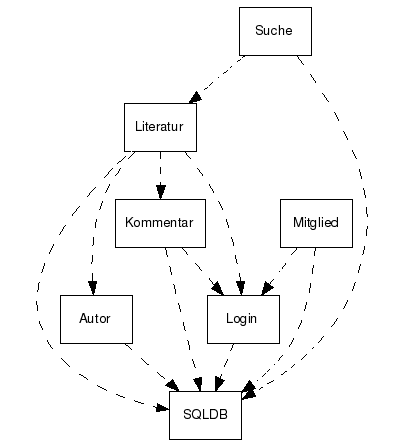
\includegraphics[scale=0.8]{../protokoll/2006_05_10.png}
					\item Generierung mit Doxygen soweit m"oglich
			\end{itemize}
			Chemnitz, 10.05.2006
			\begin{itemize}
				\item Protokolant: Simon Wunderlich
			\end{itemize}
\newpage
		\section{Protokoll 1. Pflichtkonsultation 30.05.2006}
		\subsection{Anwesende}
		\begin{itemize}
			\item Simon Wunderlich
			\item Andreas Tröger
			\item Frank Wilhelm
			\item Florian Scharl
			\item Sven Eckelmann
		\end{itemize}
		\subsection{Tagesordnung}
		\begin{itemize}
			\item Besprechung Teilbeleg 1
			\item Vorstellung Stand Teilbeleg 2
			\item Stand Projektarbeit
			\item Nächste Sitzung
		\end{itemize}
			\subsection{Besprechung Teilbeleg 1}
			\begin{itemize}
				\item fehlende Suchabfrage in Ereignistabelle und Datenkatalog
				\item kleine Fehler bei Formulierungen ({\it freier} Festplattenspeicher, Stil {\it der grafischen Oberfläche})
				\item keine Liste der Fehlercodes
			\end{itemize}
			\subsection{Vorstellung Stand Teilbeleg 2}
			\begin{itemize}
				\item Änderungsstand und Bearbeiter noch nicht aufgeführt
				\item Klassendiagramm nur ähnlich Moduldiagramm und kein UML-Klassendiagramm
			\end{itemize}
			\subsection{Stand Projektarbeit}
			\begin{itemize}
				\item Implementierung fast vollständig
				\item Systemtests am laufen bzw. in Vorbereitung
			\end{itemize}
			\subsection{Nächste Sitzung}
			\begin{itemize}
				\item Treffen am 7.6. 15:15
				\item Besprechung einzelner Punkte des 3. Belegs
			\end{itemize}
		\begin{itemize}
			\item Protokolant: Sven Eckelmann
		\end{itemize}
\newpage
		\section{Sitzungsprotokoll 07.06.2006}
		\subsection{Anwesende}
		\begin{itemize}
			\item Simon Wunderlich
			\item Andreas Tröger
			\item Frank Wilhelm
			\item Florian Scharl
			\item Sven Eckelmann
		\end{itemize}
		\subsection{Tagesordnung}
		\begin{itemize}
			\item Verteilung der Aufgaben zum 3. Teilbeleg
			\item Nächste Sitzung
			\item Nächste Pflichtkonsultation mit Betreuer
		\end{itemize}
			\subsection{Verteilung der Aufgaben zum 3. Teilbeleg}
			\begin{itemize}
			\item Programmdokumentation
			\begin{itemize}
			\item Definition der Interfaces in der Implementierungssprache -- Sven Eckelmann u. Frank 			Wilhelm
			\item Kommentierte Quelltexte -- Sven Eckelmann u. Frank Wilhelm
			\item Testplan -- Sven Eckelmann u. Frank Wilhelm
			\item Systemtest -- Sven Eckelmann u. Frank Wilhelm
			\item Abschlusseinschätzung -- Sven Eckelmann u. Frank Wilhelm
			\end{itemize}
			\item Systemhandbuch
			\begin{itemize}
			\item Installationsanleitung -- Simon Wunderlich
			\item Programm-Filesystem -- Andreas Tröger
			\item Administrationsanleitung -- Andreas Tröger
			\end{itemize}
			\item Anwenderdokumentation
			\begin{itemize}
			\item Produktzweck -- Florian Scharl
			\item Basismaschine und Ressourcenanforderungen -- Florian Scharl
			\item Nutzerklassen -- Florian Scharl
			\item Bedienungsanleitung -- Florian Scharl
			\item Helpsystem -- Florian Scharl
			\end{itemize}
			\item Übersicht über die Arbeitsaufgaben alle Teammitglieder während der gesamten Projektbearbeitung
			inkl. der Festlegungsprotokolle	-- Simon Wunderlich
			\end{itemize}
			Bemerkung: Die endgültige Festlegung erfolgt in der nächsten Sitzung nachdem jeder den Umfang 				seines Aufgabengebietes bzw. seiner Aufgabengebiete erschlossen hat.
			\subsection{Nächste Sitzung}
			\begin{itemize}
			\item Die nächste Sitzung findet am {\em 14.06.2006 um 15:15 Uhr im Raum 1/204 } statt.
			\end{itemize}
			\subsection{Nächste Pflichtkonsultation mit Betreuer}
			\begin{itemize}
			\item Die nächste Pflichtkonsultation mit Herrn Rentzsch findet am {\em 13.06.2006 um 13:10 Uhr im Raum 			1/B317 } statt.
			\end{itemize}
			Chemnitz, 07.06.2006
			\begin{itemize}
				\item Protokolant: Florian Scharl
			\end{itemize}
\newpage
		\section{Protokoll 2. Pflichtkonsultation 13.06.2006}
		\subsection{Anwesende}
		\begin{itemize}
			\item Simon Wunderlich
			\item Andreas Tröger
			\item Frank Wilhelm
			\item Florian Scharl
			\item Sven Eckelmann
		\end{itemize}
		\subsection{Tagesordnung}
		\begin{itemize}
			\item Besprechung Teilbeleg 2
			\item Vorstellung Stand Teilbeleg 3
			\item Nächste Sitzung
		\end{itemize}
			\subsection{Besprechung Teilbeleg 2}
			\begin{itemize}
				\item fehlende Trennung zwischen SQLDB-Klasse und Datenbank
				\item unklare Formulierung "Felder {\it mit Elementen} vom Typ..."
			\end{itemize}
			\subsection{Vorstellung Stand Teilbeleg 3}
			\begin{itemize}
				\item Implementierung weitgehend vollständig
				\item Tests werden fertiggestellt
				\item Anwender- und Systemdokumentation in Vorbereitung
			\end{itemize}
			\subsection{Nächste Sitzung}
			\begin{itemize}
				\item Treffen am 14.06. 15:15
				\item Besprechung einzelner Punkte des 3. Belegs
			\end{itemize}
		\begin{itemize}
			\item Protokolant: Sven Eckelmann
		\end{itemize}
\newpage
		\section{Sitzungsprotokoll 14.06.2006}
		\subsection{Anwesende}
		\begin{itemize}
			\item Simon Wunderlich
			\item Andreas Tröger
			\item Frank Wilhelm
			\item Florian Scharl
			\item Sven Eckelmann
		\end{itemize}
		\subsection{Tagesordnung}
		\begin{itemize}
			\item Besprechung Teilbeleg 3
		\end{itemize}
			\subsection{Besprechung Teilbeleg 3}
			\begin{itemize}
				\item Explizite Aufteilung noch zu erledigender Aufgaben
				\item Besprechung und Korrektur bisher vorhandener Teile
				\item Besprechung technischer Möglichkeiten zur Dokumentation der Oberfläche
				\item Archivierungsmöglichkeiten des Administrators (phpMyAdmin, mysqldump)
			\end{itemize}
		\begin{itemize}
			\item Protokolant: Sven Eckelmann
		\end{itemize}
\newpage
		\section{Sitzungsprotokoll 28.06.2006}
		\subsection{Anwesende}
		\begin{itemize}
			\item Simon Wunderlich
			\item Andreas Tröger
			\item Frank Wilhelm
		\end{itemize}
		\subsection{Tagesordnung}
		\begin{itemize}
			\item Besprechung Teilbeleg 3
		\end{itemize}
			\subsection{Besprechung Teilbeleg 3}
			\begin{itemize}
				\item Stand Aufgabenerf"ullung des Teams verglichen
				\item Details zur Administrationsanleitung besprochen
			\end{itemize}
		\begin{itemize}
			\item Protokolant: Simon Wunderlich
		\end{itemize}
\newpage


\end{document}
